\documentclass{article}
\usepackage{graphicx}
\usepackage{amsmath}
\usepackage{amssymb}
\usepackage{mathtools}
\usepackage{xcolor}
\usepackage{bm}

\usepackage{natbib}
\usepackage[hidelinks]{hyperref}
\usepackage{doi}
\usepackage{charter}
\usepackage[bitstream-charter]{mathdesign}
\usepackage[final,babel]{microtype}
\usepackage[utf8]{inputenc}
\usepackage[british]{babel}
\usepackage{csquotes}
\usepackage[T1]{fontenc}
\usepackage{siunitx}


\title{Multidimensional advection over steep terrain on a new type of Cartesian mesh \\ \TODO{(working title)}}
\author{James Shaw}

\newcommand{\iunit}{\boldsymbol{\hat \imath}}
\newcommand{\junit}{\boldsymbol{\hat \jmath}}
\newcommand{\kunit}{\boldsymbol{\hat k}}
\newcommand{\TODO}[1]{\textcolor{purple}{TODO: \emph{#1}}}

\begin{document}
\maketitle

\section{Introduction}

First, we present a multidimensional advection scheme that is computationally cheap and suitable for complex flows on arbitrary meshes.  Second, we present a new type of Cartesian mesh, the slanted cell mesh, that avoids the small cell problem associated with cut cell meshes.   We apply the advection scheme to tests over steep orography and show that accurate results are obtained on slanted cell meshes.  Finally, we challenge the multidimensional advection scheme using a test of deformational flow on a geodesic mesh.

\section{Slanted cell mesh generation}

\begin{figure}
	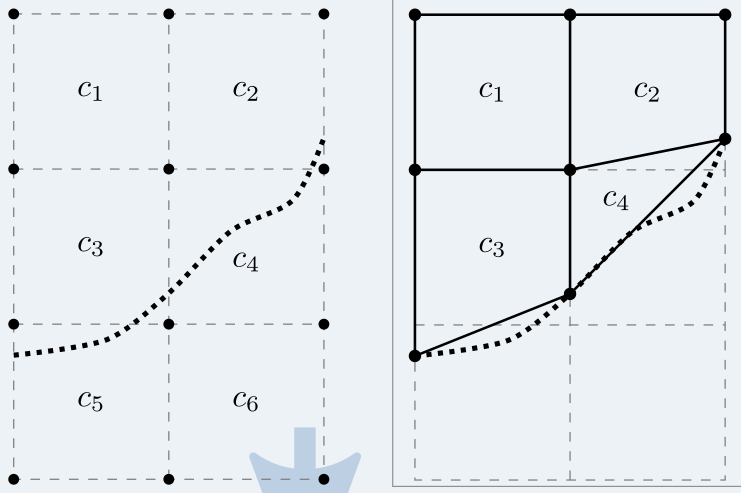
\includegraphics[width=\textwidth]{slantCellConstruction.png}
	\caption{\TODO{Before and after diagrams showing how a slanted cell mesh is constructed from a uniform quadrilateral mesh}}
\end{figure}

\begin{figure}
	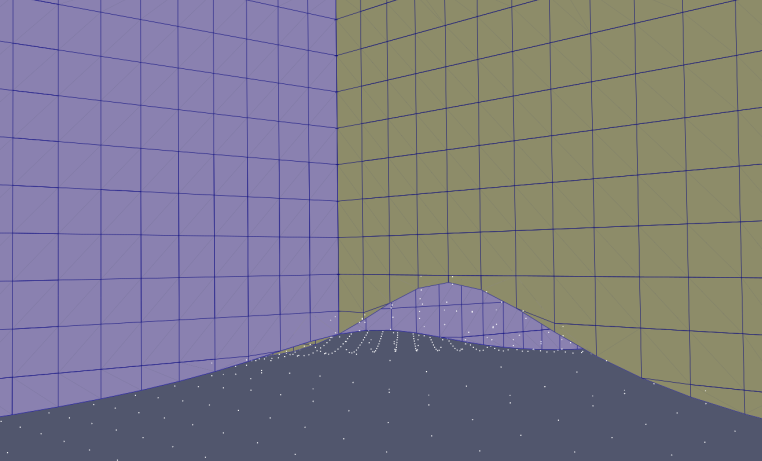
\includegraphics[width=\textwidth]{3dslices.png}
	\caption{\TODO{An example of a 3D slanted cell mesh with Alpine topography, maybe best illustrated using orthogonal cross-sections}}
\end{figure}

\begin{figure}
	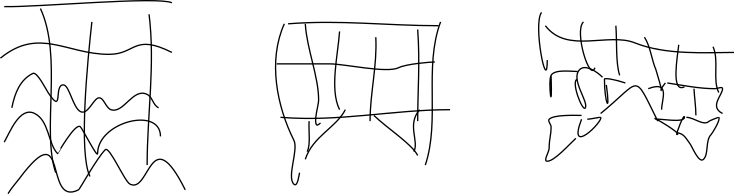
\includegraphics[width=\textwidth]{meshComparison.png}
	\caption{\TODO{examples of BTF, slanted cell and cut cell meshes with the same steep mountain profile (one of those used in the thermal advection test)}}
\end{figure}

\section{Multidimensional advection scheme}

Stability constriants:
\begin{align}
	0.5 \leq u \leq 1 \\
	0 \leq d \leq 0.5 \\
	u - d \geq \max(|p|)
\end{align}

\begin{figure}
	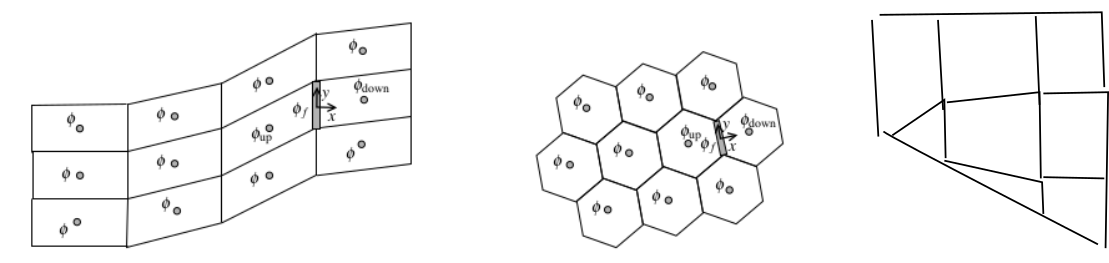
\includegraphics[width=\textwidth]{stencilConstruction.png}
	\caption{\TODO{example stencils in interior of quad and hex meshes, and example stencil near boundary of a slanted cell mesh (taken from one of the test cases)}}
\end{figure}


\section{Results}
\subsection{\TODO{Horizontal advection?}}

\subsection{Thermal advection}

Domain \SI{301}{\kilo\meter} wide, \SI{25}{\kilo\meter} high, Sch\"ar had $\Delta x = \SI{1}{\kilo\meter}, \Delta z^\star = \SI{500}{\meter}$.  Integrate \SI{18000}{\second} so that tracer initially at left hand edge of mountain has safely passed through the outlet boundary (i.e. we are in a steady-state solution).  $\Delta t = \SI{25}{\second}$ for Sch\"ar's mesh.

\begin{table}
	\begin{verbatim}
61x10		5000
121x20		2500
151x25		2000
241x40		1250
301x50		1000
451x75		 667
601x100		 500
901x150		 333
1201x200	 250
2401x400	 125
3001x500	 100
	\end{verbatim}
	\caption{\TODO{suggested $x$ cells $\times$ $z$ cells $\times \Delta t$ resolutions for thermal advection convergence tests}}
\end{table}

Mountain profile:
\begin{subequations}
\begin{align}
   h(x) &= h^\star \cos^2 ( \alpha x )
%
\intertext{where}
%
   h^\star(x) &= \left\{ \begin{array}{l l}
       h_0 \cos^2 ( \beta x ) & \quad \text{if $| x | < a$} \\
	0 & \quad \text{otherwise}
    \end{array} \right.
\end{align}
\end{subequations}
where $a = \SI{25}{\kilo\meter}$ is the mountain envelope half-width, $h_0 = \SI{6}{\kilo\meter}$ is the maximum mountain height, $\lambda = \SI{8}{\kilo\meter}$ is the wavelength, \(\alpha = \pi / \lambda\) and \(\beta = \pi / (2a)\).

$h0, a$ and $\lambda$ are chosen to give us very steep terrain, and to match those from Hilary and Yumeng's upcoming QJRMS paper.

Initial thermal profile:
\begin{align}
	\theta(z) = \theta_0 \exp \left( \frac{N^2}{g} z \right) \label{eqn:thermal-profile}
\end{align}

Velocity field:
\begin{equation}
	\Psi(x,z) = -u_0 H \frac{z - h}{H - h} \label{eqn:streamfunc-btf}
\end{equation}
where $u_0 = \SI{10}{\meter\per\second}$, which is the horizontal wind speed where $h(x) = 0$.
The horizontal and vertical components of velocity, $u$ and $w$, are then given by
\begin{align}
	u &= -\frac{\partial \Psi}{\partial z} = u_0 \frac{H}{H - h}, \quad w = \frac{\partial \Psi}{\partial x} = u_0 H \frac{\mathrm{d} h}{\mathrm{d} x} \frac{H - z}{\left( H - h \right)^2} \label{eqn:uw-btf} \\
	\frac{\mathrm{d} h}{\mathrm{d} x} &= - h_0 \left[ 
		\beta \cos^2 \left( \alpha x \right) \sin \left( 2 \beta x \right) +
		\alpha \cos^2 \left( \beta x \right) \sin \left( 2 \alpha x \right)
	\right]
\end{align}

Analytic solution:
\begin{align}
	\theta_T(x, z) = \theta_0 \exp \left( \frac{N^2}{g} z^\star(x, z) \right) 
\end{align}

\begin{figure}
	\caption{\TODO{thermal advection l2 and linf convergence plots comparing BTF, slanted cells and cut cells, cubicUpwindCPCFit and linearUpwind}}
\end{figure}

\subsection{Resting atmosphere over Alpine terrain}

\subsection{Deformational flow}
Following \citep{lauritzen2012}.  \TODO{which of the initial conditions should I use?  slotted cylinder would be the hardest}

\section{Conclusions}

The slanted cell method
\begin{itemize}
	\item avoids creating very small cells, instead creating thin cells that are long in the direction of the flow, hence alleviates the small cell problem
	\item accurately represents a hydrostatically balanced atmosphere at rest over steep Alpine terrain
	\item is straightforward compared to the cut cell method
	\item generalises to 3D
\end{itemize}

The advection scheme is
\begin{itemize}
	\item suitable for complex flows on arbitrary meshes
	\item computationally cheap at runtime, with more expensive computations depending only on the mesh geometry
	\item fourth-order convergent at best, first-order convergent at worst
	\item stable for Courant numbers up to 1
\end{itemize}

Idealised atmospheric flows over steep slopes are accurately represented using the multidimensional advection scheme without severely constraining the timestep.  The multidimensional advection scheme is suitable for complex flows on arbitrary meshes.

\section{Acknowledgements}
\TODO{Supervisors, funding bodies.  ASAM group for the mesh generator---I should ask permission to use cut cell meshes in this paper.  Shing Hing Man.}

\bibliographystyle{ametsoc2014}
\bibliography{references}

\end{document}
